\begin{naloga}{Sergio Cabello}{Teorija OR 5.9.2017}
\begin{vprasanje}
Obravnavamo manjši sudoku velikosti $4\times 4$ na sliki~\fig{}.
Vanj vpisujemo števila med 1 in 4.
Vsako število se pojavi natanko enkrat v vsaki vrstici,
vsakem stolpcu in vsakem od $4$ kvadratov velikosti $2 \times 2$,
omejenih z debelejšo črto.
Opiši celoštevilski linearni program za reševanje takega problema
oz.~za določanje, da rešitev ne obstaja.
Koliko spremenljvk in pogojev ima linearni program?

\begin{slika}
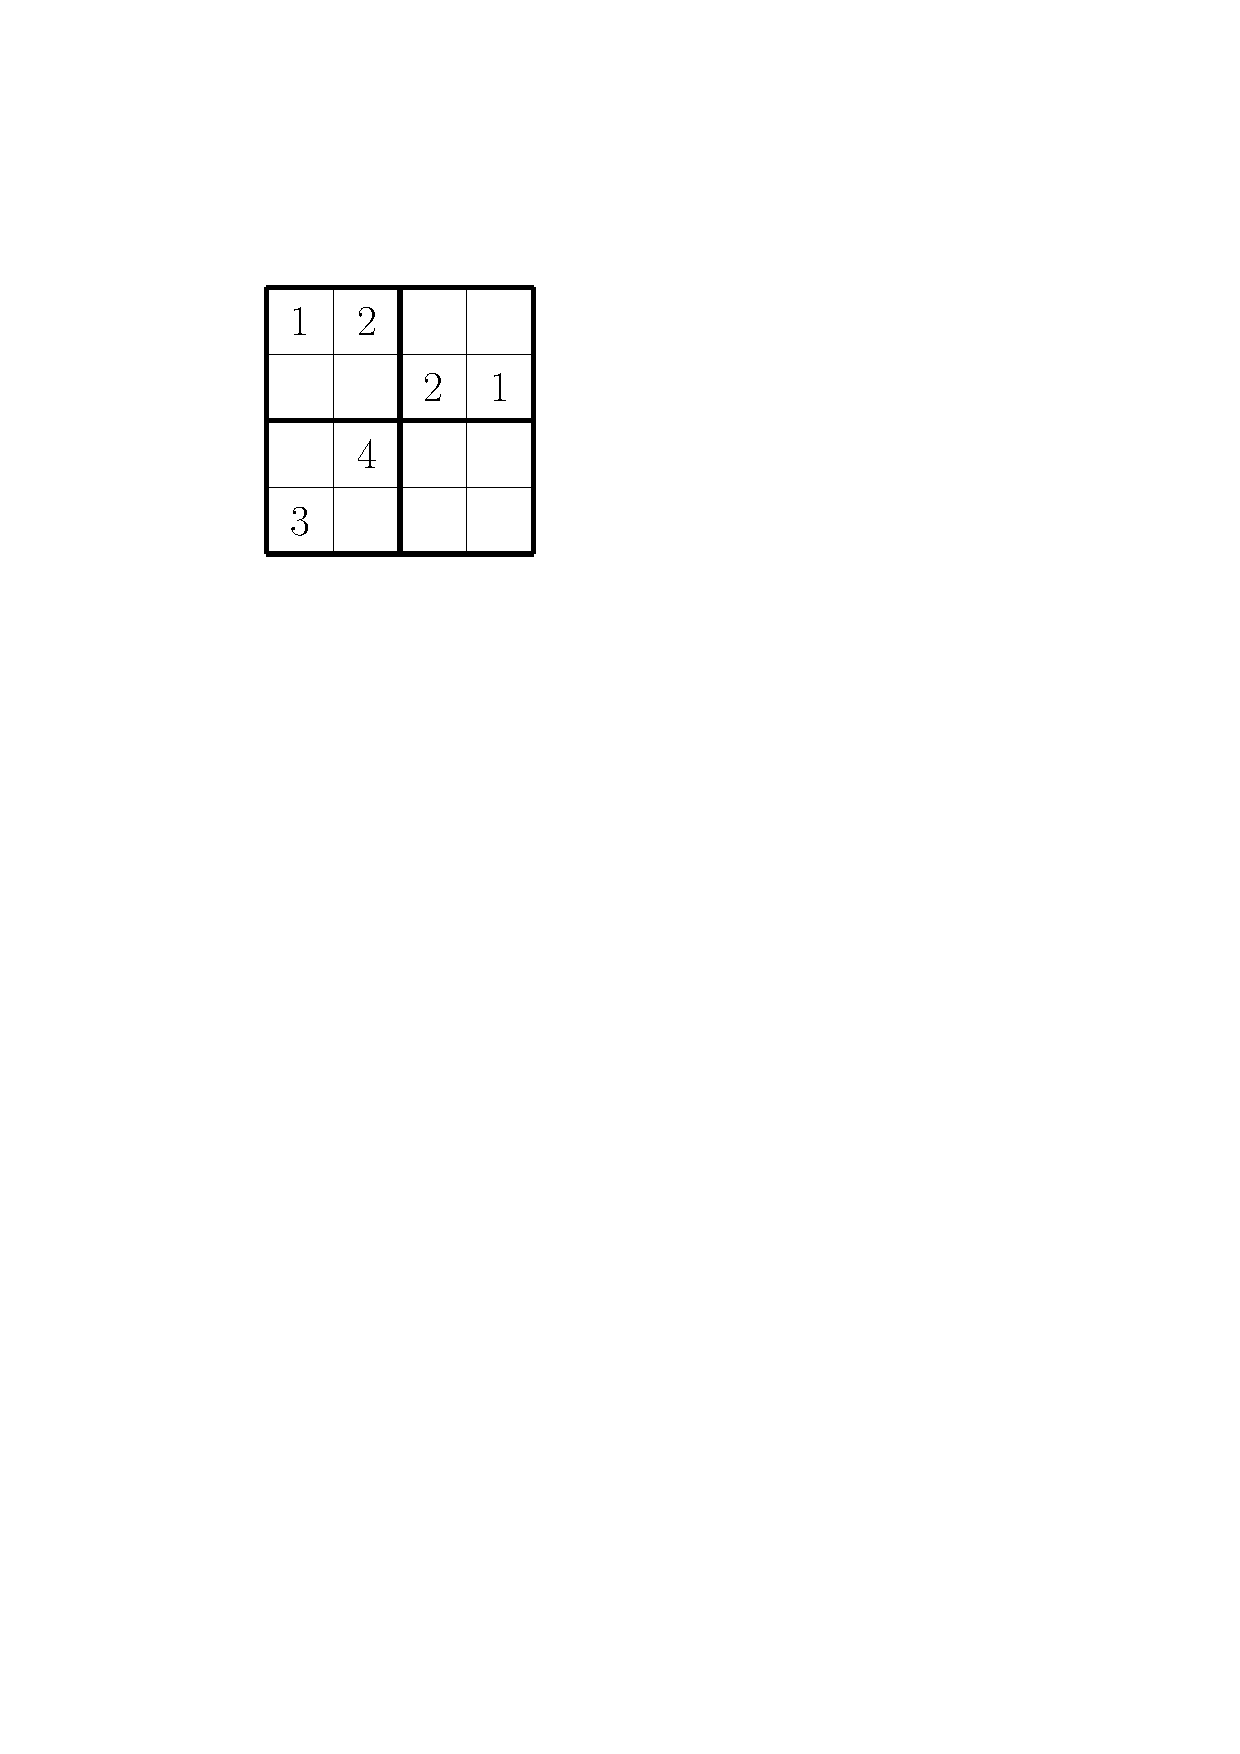
\includegraphics[scale=.7]{slike/sudoku}
\podnaslov{Primer sudokuja}
\end{slika}
\end{vprasanje}
\begin{odgovor}
\end{odgovor}
\end{naloga}
